\documentclass[11pt,answers]{exam}

% ===== Template packages + additions for plots =====
\usepackage{amsmath,yhmath}
\usepackage{verbatim}
\usepackage{graphicx}
\usepackage{amsthm}
\usepackage{amssymb}
\usepackage{fullpage}
\usepackage{hyperref}
\usepackage[parfill]{parskip}
\usepackage{tikz}
\usepackage{pgfplots}       % added for plotting the normal curves
\pagestyle{empty}

% ===== Shortcuts (optional) =====
\newcommand{\Z}{\mathbb{Z}}
\newcommand{\R}{\mathbb{R}}
\newcommand{\Q}{\mathbb{Q}}
\newcommand{\C}{\mathbb{C}}
\newcommand{\st}{\text{ such that }}
\newcommand{\E}{\mathbb{E}}
\newcommand{\Var}{\mathrm{Var}}
\newcommand{\Cov}{\mathrm{Cov}}

\begin{document}

\begin{center}
  \large \textbf{Homework \#1, ECON 107}.
\end{center}

Due by September 4th, 2025 at 1:30pm.

\begin{questions}

% ===========================
% Question 1
% ===========================
\question Suppose that $X$ is a random variable with $\E[X]=4$ and $\Var(X)=8$.
Find the expectation and variance for each transformation:
\begin{parts}
  \part $Y=X-2$.
  \part $Y=3X$.
  \part $Y=X/8$.
\end{parts}

\begin{solution}
For any constants $a\in\R$ and $b\in\R$, using the definition of expectation and variance,
\[
\E[aX+b]=a\,\E[X]+b, 
\]
\begin{align*}
\Var(aX+b) 
&= \E\!\left[(aX+b-\E[aX+b])^2\right] \\
&= \E\!\left[a^2(X-\E[X])^2\right] \\
&= a^2 \: \Var(X).
\end{align*}
Thus a constant shift $b$ changes the mean by $b$ but leaves the variance unchanged, while scaling by $a$ multiplies the variance by $a^2$.

\medskip
\textbf{Apply to each part using $\E[X]=4$ and $\Var(X)=8$:}
\begin{enumerate}
  \item[(a)] $Y=X-2$:
  \[
    \E[Y]=4-2=2,
    \qquad
    \Var(Y)=8.
  \]
  \item[(b)] $Y=3X$:
  \[
    \E[Y]=3\cdot 4=12,
    \qquad
    \Var(Y)=3^2\cdot 8=72.
  \]
  \item[(c)] $Y=X/8$:
  \[
    \E[Y]=\tfrac{1}{8}\cdot 4=\tfrac{1}{2}=0.5,
    \qquad
    \Var(Y)=\left(\tfrac{1}{8}\right)^2\cdot 8=\tfrac{1}{8}=0.125.
  \]
\end{enumerate}

\medskip
For the purposes of visualization, suppose $X\sim\mathcal{N}(4,8)$ so $\sigma_X=\sqrt{8}$. 

\newpage
% --- shared parameters for all three plots ---
\pgfmathsetmacro{\muX}{4}
\pgfmathsetmacro{\sigX}{sqrt(8)} % numeric; use pgf's sqrt

% --- Figure for (A): shift by -2 (mean from 4 to 2; variance unchanged) ---
\begin{center}
 \small\emph{(A) Subtracting 2 shifts the curve left by 2; variance unchanged.}
\begin{tikzpicture}
\begin{axis}[
  width=0.9\textwidth, height=6cm,
  xlabel={$x$}, ylabel={density},
  domain=-6:14, samples=300,
  legend cell align=left, legend pos=north east,
  axis lines=left, ymin=0
]
  % Original X ~ N(4,8)
  \addplot[thick]
    { 1/(\sigX*sqrt(2*pi)) * exp(-((x-\muX)^2)/(2*\sigX*\sigX)) };
  \addlegendentry{$X\sim\mathcal N(4,8)$}

  % Y = X - 2 has mean muX-2, same sigma
  \pgfmathsetmacro{\muA}{\muX - 2}
  \pgfmathsetmacro{\sigA}{\sigX}
  \addplot[thick,dashed]
    { 1/(\sigA*sqrt(2*pi)) * exp(-((x-\muA)^2)/(2*\sigA*\sigA)) };
  \addlegendentry{$Y=X-2\sim\mathcal N(2,8)$}

  % guide lines at the means
  \addplot[densely dotted] coordinates {(\muX,0) (\muX,0.15)};
  \addplot[densely dotted] coordinates {(\muA,0) (\muA,0.15)};
\end{axis}
\end{tikzpicture}
\end{center}

% --- Figure for (B): scale by 3 (mean 12; variance 72) ---
\begin{center}
\small\emph{(B) Multiplying by 3 stretches the distribution (variance $\times 9$) and shifts the mean to 12.}
\begin{tikzpicture}
\begin{axis}[
  width=0.9\textwidth, height=6cm,
  xlabel={$x$}, ylabel={density},
  domain=-15:40, samples=300,
  legend cell align=left, legend pos=north east,
  axis lines=left, ymin=0
]
  % Original X ~ N(4,8)
  \addplot[thick]
    { 1/(\sigX*sqrt(2*pi)) * exp(-((x-\muX)^2)/(2*\sigX*\sigX)) };
  \addlegendentry{$X\sim\mathcal N(4,8)$}

  % Y = 3X has mean 3*muX, sd 3*sigX
  \pgfmathsetmacro{\muB}{3*\muX}
  \pgfmathsetmacro{\sigB}{3*\sigX}
  \addplot[thick,dashed]
    { 1/(\sigB*sqrt(2*pi)) * exp(-((x-\muB)^2)/(2*\sigB*\sigB)) };
  \addlegendentry{$Y=3X\sim\mathcal N(12,72)$}

  % guide lines at the means
  \addplot[densely dotted] coordinates {(\muX,0) (\muX,0.15)};
  \addplot[densely dotted] coordinates {(\muB,0) (\muB,0.15)};
\end{axis}
\end{tikzpicture}
\end{center}

% --- Figure for (C): scale by 1/8 (mean 0.5; variance 1/8) ---
\begin{center}
\small\emph{(C) Dividing by 8 compresses the distribution (variance $\times \tfrac{1}{64}$) and shifts the mean to $0.5$.}
\begin{tikzpicture}
\begin{axis}[
  width=0.9\textwidth, height=6cm,
  xlabel={$x$}, ylabel={density},
  domain=-2:5, samples=300,
  legend cell align=left, legend pos=north east,
  axis lines=left, ymin=0
]
  % Original X ~ N(4,8)
  \addplot[thick]
    { 1/(\sigX*sqrt(2*pi)) * exp(-((x-\muX)^2)/(2*\sigX*\sigX)) };
  \addlegendentry{$X\sim\mathcal N(4,8)$}

  % Y = X/8 has mean muX/8, sd sigX/8
  \pgfmathsetmacro{\muC}{\muX/8}
  \pgfmathsetmacro{\sigC}{\sigX/8}
  \addplot[thick,dashed]
    { 1/(\sigC*sqrt(2*pi)) * exp(-((x-\muC)^2)/(2*\sigC*\sigC)) };
  \addlegendentry{$Y=\tfrac{X}{8}\sim\mathcal N(0.5,\,1/8)$}

  % guide lines at the means
  \addplot[densely dotted] coordinates {(\muX,0) (\muX,0.5)};
  \addplot[densely dotted] coordinates {(\muC,0) (\muC,0.5)};
\end{axis}
\end{tikzpicture}
\end{center}

\end{solution}

% ===========================
% Question 2
% ===========================
\newpage
\question Let $X=1$ if there is a recession in the next four quarters and $X=0$ otherwise; 
let $Y=1$ if unemployment exceeds $7\%$ and $Y=0$ otherwise. 
The joint probabilities are
\[
\begin{array}{c|cc}
  & X=1 & X=0\\\hline
Y=1 & 0.4 & 0.1\\
Y=0 & 0.1 & 0.4
\end{array}
\]

\begin{parts}

\part \textbf{Marginal pmf of $X$.}
\begin{solution}
$\Pr\,(X=1)=0.4+0.1=0.5$ and $\Pr\,(X=0)=0.1+0.4=0.5$.
\end{solution}

\part \textbf{$\E[Y]$.}
\begin{solution}
Since $Y\in\{0,1\}$, $\E[Y]=\Pr\,(Y=1)=0.4+0.1=0.5$.
\end{solution}

\part \textbf{$\E[Y\mid X=0]$.}
\begin{solution}
$\E[Y\mid X=0]=\Pr\,(Y=1\mid X=0)=\dfrac{\Pr\,(Y=1,X=0)}{\Pr\,(X=0)}=\dfrac{0.1}{0.5}=0.2$.
\end{solution}

\part \textbf{$\Var(Y\mid X=0)$.}
\begin{solution}
Conditional on $X=0$, $Y\sim\text{Bernoulli}(p)$ with $p=0.2$, so $\Var(Y\mid X=0)=p(1-p)=0.2\cdot 0.8=0.16$.
\end{solution}

\part \textbf{$\Cov(X,Y)$.}
\begin{solution}
$\Cov(X,Y)=\E[XY]-\E[X]\E[Y]$. Here $\E[XY]=\Pr\,(X=1,Y=1)=0.4$, $\E[X]=0.5$, and $\E[Y]=0.5$, so $\Cov(X,Y)=0.4-0.25=0.15$.
\end{solution}
\end{parts}

\newpage
\question Graphing and examining CEPR data.

\begin{parts}

\part Build a nice table.
\small
\verbatiminput{logs/problem3_3a.log}	
\include{problem_3a_table}

\part Build a box plot.
\small
\verbatiminput{logs/problem3_3b.log}	
\includegraphics[width=0.9\linewidth]{figures/problem_3b_boxplot.png} \\
The appendix figure is virtually identical.

\part Analyze variables for issues.
\small
\verbatiminput{logs/problem3_3c.log}	

\part De-string hhid2.
\small
\verbatiminput{logs/problem3_3d.log}	
	
\end{parts}

\newpage
\question Cost of best management practices (bmp) for stormwater management.

\begin{parts}

\part Find the correlation coefficient between costbmp and gallons, interpret it.
\small
\verbatiminput{logs/problem4_4a.log}	

\part Draw five random 20\% samples and compare their output correlations to the correlation over the entire sample.
\small
\verbatiminput{logs/problem4_4b.log}	
	
\part Create a binned visual.
\small
\verbatiminput{logs/problem4_4c.log}
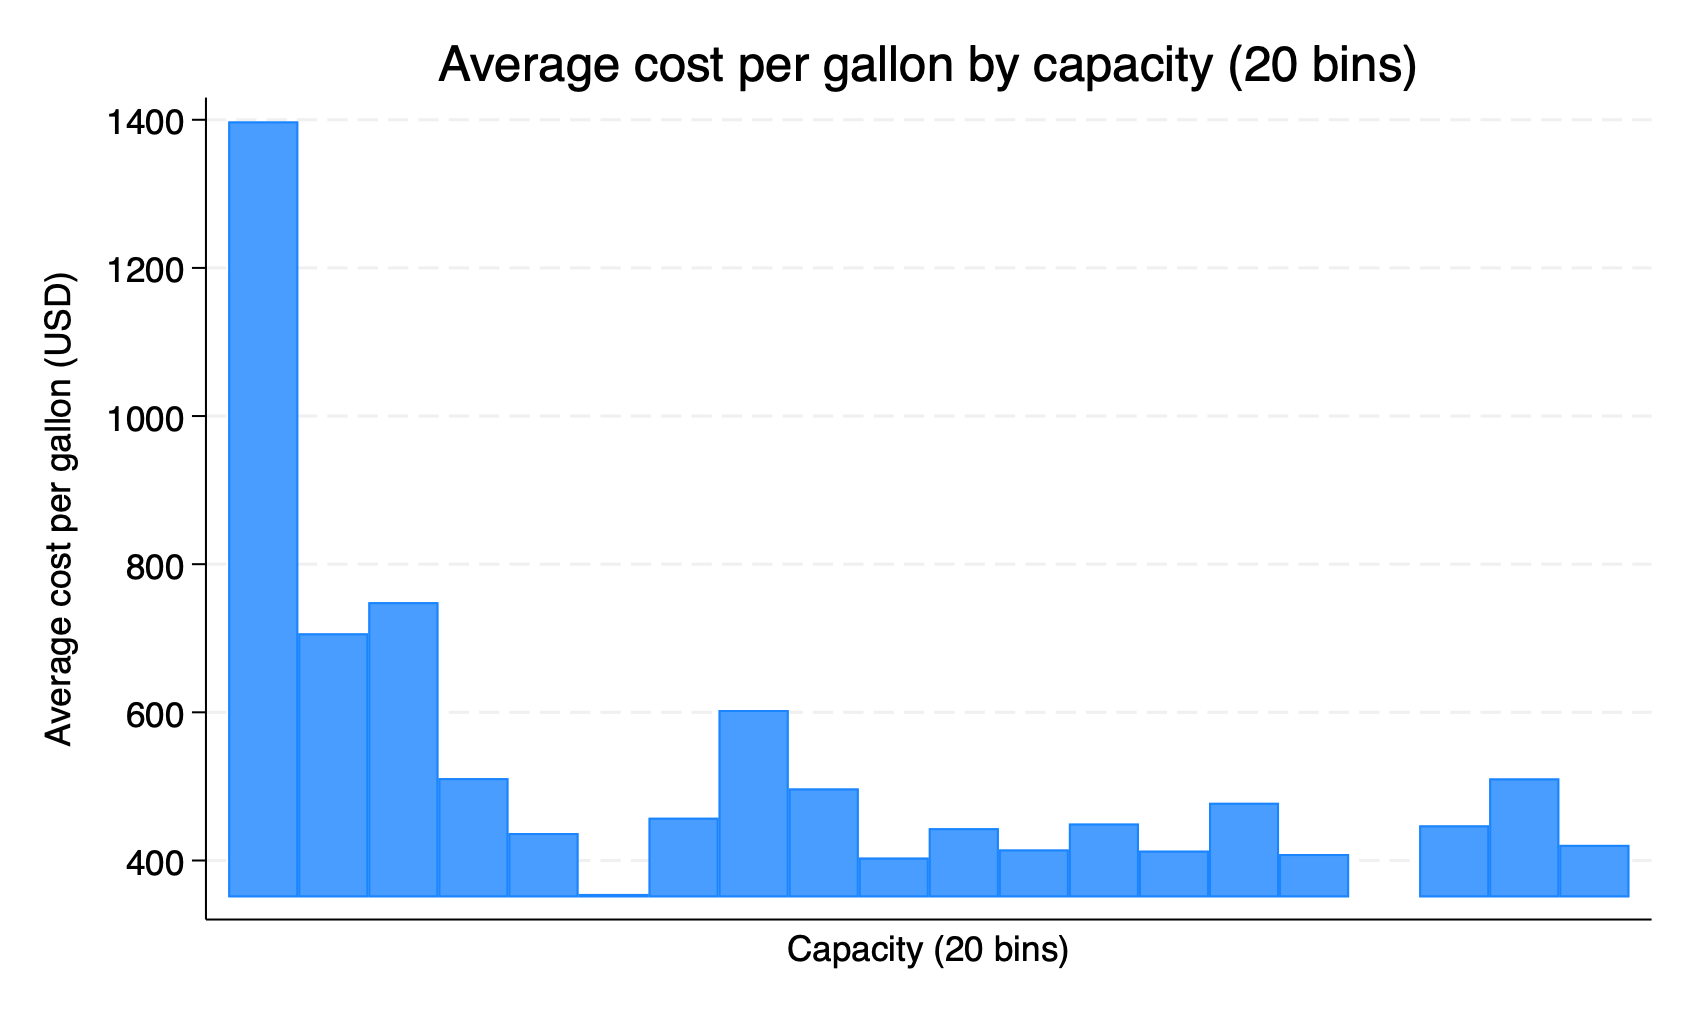
\includegraphics[width=0.95\linewidth]{figures/problem_4c_cpg_by_bin.png}

\end{parts}

\question Summary of Undergraduate Econometrics paper.

In "Fertility Policies and Women’s Education in Contemporary China: A Study of the Two-Child Policy's Effects," published in the Volume 14 of the Berkeley Economic Review, Monica Wu investigates the extent to which China's shift from the one-child policy to the selective (2014) and later universal (2016) two-child policy affected women's educational investment. I chose this paper because I believe that its empirical strategy could be useful for my paper idea.

In terms of data, the analysis uses the China Family Panel Studies (CFPS)---a national survey covering 25 provinces (approx. 80\% of China's population). Wu works primarily with survey waves spanning from 2012 to 2020 and a sample of $n=31{,}741$ woman-year observations. Notably, women's educational investment is operationalized as log household educational expenditures that are primarily attributed to the mother. Other key variables from the data include demographics (age, health), household economics (log per-capita income, net assets, family size), and residence (urban/rural). A table of summary statistics is reproduced below:

  \small
  \begin{tabular}{lrrrrrr}
    \hline
    \textbf{Variable name} & \textbf{Obs} & \textbf{Mean} & \textbf{Std. Dev.} & \textbf{Median} & \textbf{Min} & \textbf{Max} \\
    \hline
    Log of Educational Fees                 & 31741 & 0.0333 & 0.5268 & 0       & 0       & 10.5967 \\
    DID Estimator                           & 31741 & 0.1541 & 0.3610 & 0       & 0       & 1       \\
    Log of Family Scale                     & 31741 & 1.4254 & 0.3862 & 1.3863  & 0       & 2.3026  \\
    Log of Per Capita Net Family Income     & 31741 & 8.9654 & 1.1658 & 9.1226  & 4.9618  & 11.2730 \\
    Net Family Assets                       & 31741 & 349488.4 & 620604.6 & 160426 & -109749 & 4325800 \\
    Log of Age                              & 31741 & 3.6699 & 0.2232 & 3.7136  & 3.1355  & 4.0431  \\
    Native Status                           & 31741 & 0.9109 & 0.2849 & 1       & 0       & 1       \\
    Health Status                           & 31741 & 2.7786 & 1.2488 & 3       & 1       & 5       \\
    Urban Residency Indicator               & 31741 & 0.4485 & 0.4974 & 0       & 0       & 1       \\
    \hline
  \end{tabular}

Using this data, Wu estimates a two-way fixed-effects difference-in-differences (TWFE-DiD) model at the woman-year level. More specifically, the model estimates
\[
\log(\text{EduFee}_{it})
= \beta\,(\text{Treat}_i \times \text{Post}_{it})
+ \gamma\,\text{Treat}_i
+ \delta\,\text{Post}_{it}
+ X_{it}'\theta
+ \alpha_i + \tau_t + \varepsilon_{it},
\]
where \(\alpha_i\) and \(\tau_t\) are individual (time-invariant heterogeneity) and year (shocks) fixed effects respectively, \(X_{it}\) are time-varying controls (e.g. income, assets), and \(\beta\) is the DiD parameter of interest. The `Treatment' term is used to model the gradual rollout of the two-child policy by capturing eligibility for the selective (2014) wave. The `Post' term addresses the post-universal (after 2016) implementation period. Various robustness checks, inclusive of fertility-age cutoffs and heterogeneity (Han vs. minority), are also presented.

Across specifications, the $(\text{Treat}_i \times \text{Post}_{it})$ coefficient ranges from $-0.028$ to $-0.062$, implying a 2.8\%-6.2\% reduction in women's educational expenditures after the two-child policy relative to comparable controls. Model fit is modest, but F-statistics are large. Interestingly, the $\text{Treat}_i$ term coefficient is positive, $(\approx 0.035-0.077)$, indicating higher baseline spending among the treated group prior to policy implementation.

Owing to the battery of controls implemented, and the fact that the policy changes of interest are plausibly exogenous to any single woman, the central coefficients represent plausibly causal estimates of the effect of the two-child policy's effect on women's educational spending. The primary remaining difficulty is that educational spending in the dataset Wu uses is measured at the household level, which means that we have a causal estimate of a policy effect on household education spending associated with mothers, not necessarily mothers' schooling per se, especially if mothers spend on their children's education.

\question Description of Paper Idea.

The Servicemen's Readjustment Act of 1944 (GI Bill) is widely understood to have powered mid-century upward mobility by expanding access to higher education and subsidizing homeownership for returning soldiers. The causal effects on schooling and home buying are well documented: World War II service substantially raised veterans' college attendance and completion (Bound and Turner 2002; 2003), and the GI Bill’s generous mortgage guarantees increased homeownership by easing down-payment and amortization constraints (Fetter 2013). It is therefore all the more notable that the historical record demonstrates that discrimination against Black WWII veterans in the use of GI Bill housing benefits was widespread. 

Archival and historical scholarship shows how local, lender, and federal underwriting practices jointly limited access for Black borrowers. Onkst (1998) documents that, despite formal eligibility, Black veterans in the Deep South rarely secured VA-backed mortgages. Woods (2013) provides corroborating evidence in the Northeast, noting that fewer than 100 of 67,000 GI Bill–backed mortgages in the New York-New Jersey region went to non-white veterans. The mechanisms have been mapped in detail: federal appraisal regimes and local banking practices embedded racialized risk assessments into underwriting (Winling and Michney 2021), and federal insurance programs systematically avoided lower-income, often minority, urban neighborhoods (Fishback, Rose, and Snowden 2024).

The same policy that functioned as an engine of mobility for many white veterans was implemented in ways that systematically restricted Black veterans' access to the housing benefit---foreclosing a central channel of wealth accumulation---thereby embedding disparities in neighborhood opportunity structures that plausibly persist to the present. Establishing the magnitude and persistence of those effects is essential for understanding a contributing factor to the historical roots of contemporary racial gaps in homeownership and  neighborhood quality.

In my project, I will aim to use census data from IPUMS to estimate the causal impact of Black veterans' exclusion from GI Bill housing benefits on neighborhood ownership composition for the veterans themselves and for their progeny across 1950-2020. The central research questions are thus:

\begin{enumerate}
	\item How does the denial of GI Bill housing benefits to Black WWII veterans affect homeownership outcomes and the ownership composition of the neighborhoods they inhabited in the postwar decades?
	\item How does the initial denial of housing benefits to Black veterans affect the homeownership and neighborhood outcomes of their progeny over time, through 2020?
\end{enumerate}

In terms of preliminary empirical strategy, I will use nationwide IPUMS microdata from the decennial censuses (1950-2020) to construct county-level panels of homeownership rates, housing values, and racial composition, along with micro-level indicators for veteran status, race, and household structure. The first set of regressions will use a differences-in-differences approach with fixed-effects controls, echoing Wu (2025):
\[
\text{Homeownership}_{ict}
= \beta_1\,(\text{Black Veteran})_{ict} + \beta_2\,(\text{White Veteran})_{ict} + \mathbf{\theta}X_{ict} + \mu_c + \tau_t + \varepsilon_{ict},
\]
where $\mu_c$ and $\tau_t$ are country and census-year fixed effects respectively, $X_{ict}$ captures age, education, marital status, and occupation. Thus, we are interested in $(\beta_1-\beta_2)$.

\begin{thebibliography}{99}

\bibitem{BoundTurner2002}
Bound, John, and Sarah Turner. 2002. ``Going to War and Going to College: Did World War II and the G.I. Bill Increase Educational Attainment for Returning Veterans?'' \textit{Journal of Labor Economics} 20(4): 784--815. https://doi.org/10.1086/342012.

\bibitem{TurnerBound2003}
Turner, Sarah, and John Bound. 2003. ``Closing the Gap or Widening the Divide: The Effects of the G.I. Bill and World War II on the Educational Outcomes of Black Americans.'' \textit{The Journal of Economic History} 63(1): 145--177. https://doi.org/10.1017/S0022050703001761.

\bibitem{Fetter2013}
Fetter, Daniel K. 2013. ``How Do Mortgage Subsidies Affect Home Ownership? Evidence from the Mid-Century GI Bills.'' \textit{American Economic Journal: Economic Policy} 5(2): 111--147. https://doi.org/10.1257/pol.5.2.111.

\bibitem{Onkst1998}
Onkst, David H. 1998. ```First a Negro \ldots\ Incidentally a Veteran': Black World War Two Veterans and the G.\,I. Bill of Rights in the Deep South, 1944--1948.'' \textit{Journal of Social History} 31(3): 517--543. https://doi.org/10.1353/jsh/31.3.517.

\bibitem{Woods2013}
Woods II, Louis Lee. 2013. ``Almost `No Negro Veteran \ldots\ Could Get a Loan': African Americans, the GI Bill, and the NAACP Campaign Against Residential Segregation, 1917--1960.'' \textit{The Journal of African American History} 98(3): 392--417. https://doi.org/10.5323/jafriamerhist.98.3.0392.

\bibitem{WinlingMichney2021}
Winling, LaDale C., and Todd M. Michney. 2021. ``The Roots of Redlining: Academic, Governmental, and Professional Networks in the Making of the New Deal Lending Regime.'' \textit{Journal of American History} 108(1): 42--69. https://doi.org/10.1093/jahist/jaab066.

\bibitem{FishbackEtAl2024}
Fishback, Price V., Jonathan D. Rose, Kenneth A. Snowden, and Thomas Storrs. 2024. ``New Evidence on Redlining by Federal Housing Programs in the 1930s.'' \textit{Journal of Urban Economics} 141: 103462. https://doi.org/10.1016/j.jue.2022.103462.

\bibitem{IPUMS2025}
Ruggles, Steven, Sarah Flood, Matthew Sobek, Daniel Backman, Grace Cooper, Julia A. Rivera Drew, Stephanie Richards, Renae Rogers, Jonathan Schroeder, and Kari C.\,W. Williams. 2025. \textit{IPUMS USA} [dataset]. Minneapolis, MN: IPUMS. https://doi.org/10.18128/D010.V16.0.

\end{thebibliography}


\end{questions}

\end{document}
